
\section{Background}\label{sec:rw}

\subsection{Domain modeling of Robot Hardware and Model Metrics}

Not too surprisingly, the Object Management Group (OMG) has taken an interest in standardizing the domain of robotics in the establishment of the Robotics Domain Task Force (RDTF) \cite{omg}. They have a small set of platform independent models (PIM) and platform specific models (PSM) \cite{rtc08,sdo08,rls10} for robotics defined in terms of UML. None, however, focus on the modeling of the kinematics and dynamics of robots. The researchers in \cite{schlegel09,Steck2010} used Eclipse Modeling Framework to deploy application software to different device-framework pairs. One \cite{schlegel09} used models for a P3DX robot and a QFIX-based robot to for several different platforms, including Player, Microsoft Robotics Studio, and SmartSoft \cite{smartsoft}. Statecharts \cite{Harel1988} were used to define robotic behavior. The other \cite{Steck2010} proposed SMARTMARS, a meta-model derived from SMARTSOFT to use for modeling and analysis of robots. A separate researcher \cite{Trojanek2011} used a similar approach to build a subsumption-based robot architecture which was deployed to a NXT Mindstorms robot. These approaches represent an alternative to working directly in a domain-specific language, instead relying on well-understood standards like UML. There are some drawbacks to this approach as at least some textual representation is still needed for the model to be serialized and passed over the network. As well, textual representations tend to simplify visual models as they do not need to include user interfaces aspects of visual models such as the position of a model element on the computer screen. However, structured visual formalisms may be compiled into a domain-specific language which could turn out to be a preferred way to model particular robots.

A secondary goal for this project will involve evaluating the proposed model in reference to other existing models and to assess the progress of the model as it grows in the long-term. Therefore, one shall define a set of metrics to assess model growth and quality, and possibly also the size in relation to other models (other models in this case being the implied models used by the aforementioned frameworks). To achieve a reference frame for how this might be accomplished, a short literature review was conducted on the current view of metrics at the model level, useful for this project. Mohagheghi presents a survey of the state of model metrics as a part of an ongoing research effort in model quality metrics \cite{Mohagheghi2009}. The paper presents six general goals for measurement at the model level which should serve as the inspiration for the metrics used to evaluate a model. The ideas of Lange on model size \cite{Lange2007} are also presented, in particular dealing with UML models. Lange proposes a specific metric for UML relative size, which could be used to measure the size of the proposed robot model against existing description models. In \cite{Wu2010}, the authors present their perception of model metrics for DSLs, offer a classification of the types of effort they believe are encountered when working within a domain-specific model (DSM), the two basic types being Development Effort and Runtime Effort. Within the context of this project, the metrics which measure Development Effort are most interesting, particularly those which measure Modeling Effort, the effort involved in developing a DSML model, and Cognitive Effort, the cognitive effort required to do so. They use a weighted sum to approximate the size of a model as a means to measure modeling effort. This metric should be fairly sufficient for calculating an inexact model size, and it should translate well between different models. Another interesting metric they use is the closeness of mapping ratio (COMR) which they used the ratio of the number of problem-level language primitives to the number of solution-level primitives which do not have mapping to the problem domain. This metric is interesting because it provides insight to the disconnect between the problem domain and the solution domain. However, to actually implement this metric would require a classification of any existing language to be benchmarked against and could be expensive time-wise. The authors also mentioned other metrics which are useful when evaluating imperative languages, however this project will focus on building a declarative language so they will not be so directly applicable. The author in \cite{Sprinkle2010} considers a new approach to estimating a model complexity via the analysis of the meta-model which defines it. This could solve the problem of evaluating complexity in a purely declarative model like RDIS.

\subsection{Hardware descriptions in existing frameworks}
%Many approaches have been used to increase reusability of software artifacts.  Player/Stage drivers can be used directly in ROS \cite{quigley2009}.  Microsoft Robotics Studio uses a service-based paradigm to abstract data sources.  Orocos \cite{Bruyninckx2001} leverages the component design to package related software into a reusable piece.  Carmen \cite{Montemerlo2003}, LCM \cite{Huang2009} and ROS \cite{quigley2009} abstract the message content from the message generation by providing a transport between modules with self-describing data.  These approaches utilize fairly advanced computer science paradigms of distributed development (utilized by many Linux-based open source projects).  Unfamiliarity with these paradigms may discourage many researchers, hobbyists and students from attempting to reuse software, even when it can teach domain specific concepts.

\begin{figure*}[thpb]
      \centering
      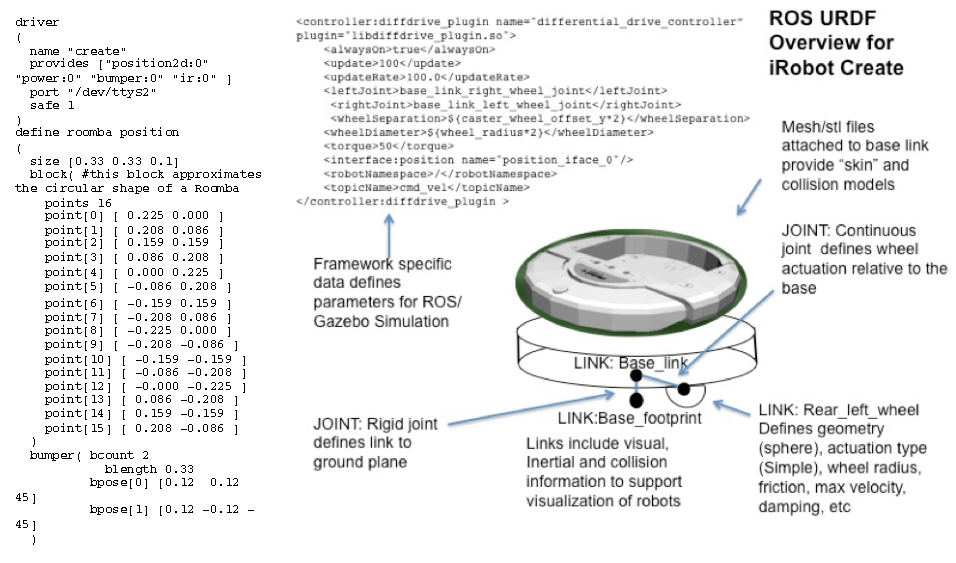
\includegraphics[width=5in]{images/URDFPS.pdf}
      \caption{Sample device descriptions within frameworks.}
      \label{psurdf}
\end{figure*}



Many frameworks use a declarative description of the robots.  Player/Stage \cite{vaughan2007} is both a 2D simulator and a robot control framework.  Robot description files are broken into two pieces: 1) a 2D description of the robot and its sensors(Figure \ref{psurdf}: right) and 2) a set of interfaces that abstract the data produced by hardware to a standard format.  The description, used for simulating the robot, consists of a polygon-based footprint with sensor locations marked. Actuation and sensor characteristics along with parameters for simplified error models are used to complete the model of the robot.  A domain-specific set of classes and message types describe what data can be obtained or how the robot can be manipulated including position (pose2d) and distance to other objects (single point is range, multipoint is laser).  The classes and message types represent the interface that abstracts the robot hardware to the data that it can produce or consume.  Writing software to the interfaces that a robot can utilize (rather than the specific robot) allows software to be written either for a simulated robot or a real robot, which in turns eases the transition from simulation to physical implementation.

ROS \cite{quigley2009} targets a 3D simulation framework (Gazebo) and more sophisticated intelligent controller, which require a more rigorous description.  UDRF (Uniform Robot Description Format) provides a 3D physical description broken into links and joints to facilitate not only mobile robots but manipulators as well (Figure \ref{psurdf}: right).  Geometric bounding boxes and meshes allow for collision detection and realistic visualization.  Like Player Stage, ROS utilizes a message-based model to decouple data providers from data producers.  Ideally robots that provide and consume similar data types can be controlled similarly.  Unlike Player Stage, URDF not only serves as a mechanism for simulating robots but also allows for the visualization of real robots in both real-time and off-line (through saved messages). 

URBI \cite{Baillie2005} is a domain specific language for robot applications. It is a platform which controls robots. Its language, urbiscript, has native syntax for parallel and event-driven constructs. This gives it high expressivity for solving problems common in robots. As an example, urbiscript can easily natively express ``when my left arm stops moving, start moving the right arm.'' However, the limitation in URBI is that it is another platform. It expects that the ``UObject'' needed to control the robot exists. Also, URBI focuses only on robotic control, however it can tie into simulators to be used as a control module for the simulation.

The authors in \cite{Schultz2007} present a domain specific language for the control of a novel robot. The ATRON self-configurable robot is composed of several independent modules which can be assembled in different manners to create a robot whose function changes according to how the modules are connected. They use the example of a car configuration in their paper. Their language is role-based, meaning a module can deduce its role by examining its own connectivity. The advantage to this type of description is that it allows the reuse of one behavior description for several configurations of ATRON modules. For example, a description file that represents a car may be used for four-wheel or six-wheel configurations. This is an interesting abstraction for application code, however it has the same problem as URBI, in that a platform-specific module must be created so that a robot may communicate with the framework.  Although the literature reveals very few attempts at using DSLs for hardware device drivers, Thibault et al report the creation of efficient video device drivers using a novel DSL \cite{Thibault1999}.  

A select number of robot control frameworks move beyond visualization information and relevant interface declaration in the hardware description.  PREOP, an Alice-based programming interface \cite{cooper2000,Wellman2009,Anderson} for robots takes this paradigm further.  Not only is 3D visualization information supplied but also the programming interface is completely specified by the selection of the robot object.  This is accomplished by linking the real-time control mechanism and exposed API available to the user within the robot object.  

All robotic architectures require that the user provides information regarding the target hardware devices and the resulting data at development time in absentia of the hardware.  Two problems result from this process: 1) users must understand the hardware and resulting data and 2) encode the hardware details properly in the framework of choice.   A mechanism that provides the user with the details of available resources could remove this step and the associated issues with attempting to properly characterize the hardware.  More importantly, self-describing hardware could lessen both frustration and the need for in-depth hardware knowledge on the part of the user.  

\subsection{RDIS (Robot Device Interface Specification)}
We propose a new paradigm where knowledge of the hardware mechanism is embedded in the hardware, rather than declared in software.  RDIS (Robot Device Interface Specification) has three purposes: 1) provide enough information for simulation and visualization of hardware and controllers, 2) declaratively specify the mechanism for requesting data and actuation, and 3) inform users of standard message types that can be obtained from the hardware to facilitate connection to existing frameworks through discovery.  The challenge in successfully defining the RDIS is in creating a model that captures the generalizable aspects of robots and provides a mechanism to specialize the aspects that vary.

RDIS relies upon the relatively invariant nature of mobile robots.  Although some robots are built for a specific task, general use robots within education and research communities tend to leverage designs that provide closed loop inverse kinematic solutions; differential drive being part of this class of robots.  In addition, many robots including the popular Mobile Robots Pioneer class, iRobot Creates, K-Team robots, Erratic ER-1, White Box Robotics Model 914, Ar.Drones, and BirdBrain Finches
\monica{[references?]}
contain an embedded firmware controller that accepts commands via a serial, Bluetooth, WiFI or USB interface rather than require the users to download a program to onboard memory.  Even robots that require a local software program to run have modes where the local software program presents an API to an external computer (i.e. Lego Mindstorms via Lejos and E-Puck).  In both of these cases, the users create an autonomous controller program that communicates with the firmware to affect actuation and to obtain sensor information.  

%RDIS relies upon two assumptions: 1) robot devices typically contain firmware that manages all hardware resources and exposes access to off-board programs via APIs and 2) many robot devices employ mechanisms that can be generalized and managed at an abstract level.  Not all robot devices contain a firmware that enables off-board programming.  However, this is an assumption that is used within many frameworks (as most frameworks are too processor and memory intensive to run on the limited resources available to on-board controllers).  In addition, firmware often chooses to hide the complexity of managing hardware resources in real time by exposing an API to access and manipulate hardware.

The RDIS specification can be defined as DSL that is used to program robots at a higher, domain-specific level.  In the application of robots, the existence of firmware (not programming hardware directly) simplifies the process.  Designing a declarative specification for robot hardware requires a solid domain model of the hardware connection and services that are provided.  Domain models, when designed properly, can be somewhat invariant to changes and can provide a stable basis for deciding the structure and parameters of the specification.  %Figure \ref{circles} shows a typical implementation of mobile robot device driver.   

The preliminary artifacts generated in this approach include RDIS specifications and grammars that generate a command line program and a ROS driver \cite{Anderson2012}.  The initial scope of this research focuses on a set of domain concepts that represent popular platforms and devices and therefore are present in most frameworks as an abstraction.   The current set of domain concepts include {\sc differential drive} and {\sc range}.   Differential drive robots (robots with two opposing wheels on a single axis) are controllable using linear and rotational velocity.   Acknowledging differential drive explicitly allows for an easier parameterization through state variables that denote odometry resolution, wheel size, offset of axis and wheel base.  While some frameworks explicitly recognize differential drive as a kinematic design (Player), others group all platforms under a single fully expressive interface where the user must know which dimensions are controllable.  For example, within the ROS system, a {\sc Twist} message type is used to provide control commands to a differential driver robot through linear and angular velocity.  The ROS template (discussed in more detail in \cite{Anderson2012}) maps each domain concept to the appropriate programming paradigm, which in this case is a subscription to the {\sc Twist} message and a callback handler that contains the code to map the {\sc Twist} message parameters to the {\sc setSpeed} firmware primitive.   A preliminary RDIS has been implemented for the Finch robot from Bird Brain and the K-Team Koala\cite{Anderson2012}.  In this design, a JSON-based description file is used (although any syntax can be used including XML).  The intermediate product is an abstract syntax tree that represents the robot details in a domain specific model.  This intermediate format can be further processed to verify conformance to the specification.  End products such as framework specific device drivers or stand-alone servers are generated from the verified syntax tree using templates that format data based on the model. 


